\begin{wrapfigure}{r}{0.4\linewidth}
\centering
\begin{subfigure}{.46\linewidth}
\centering
\raisebox{0.1cm}{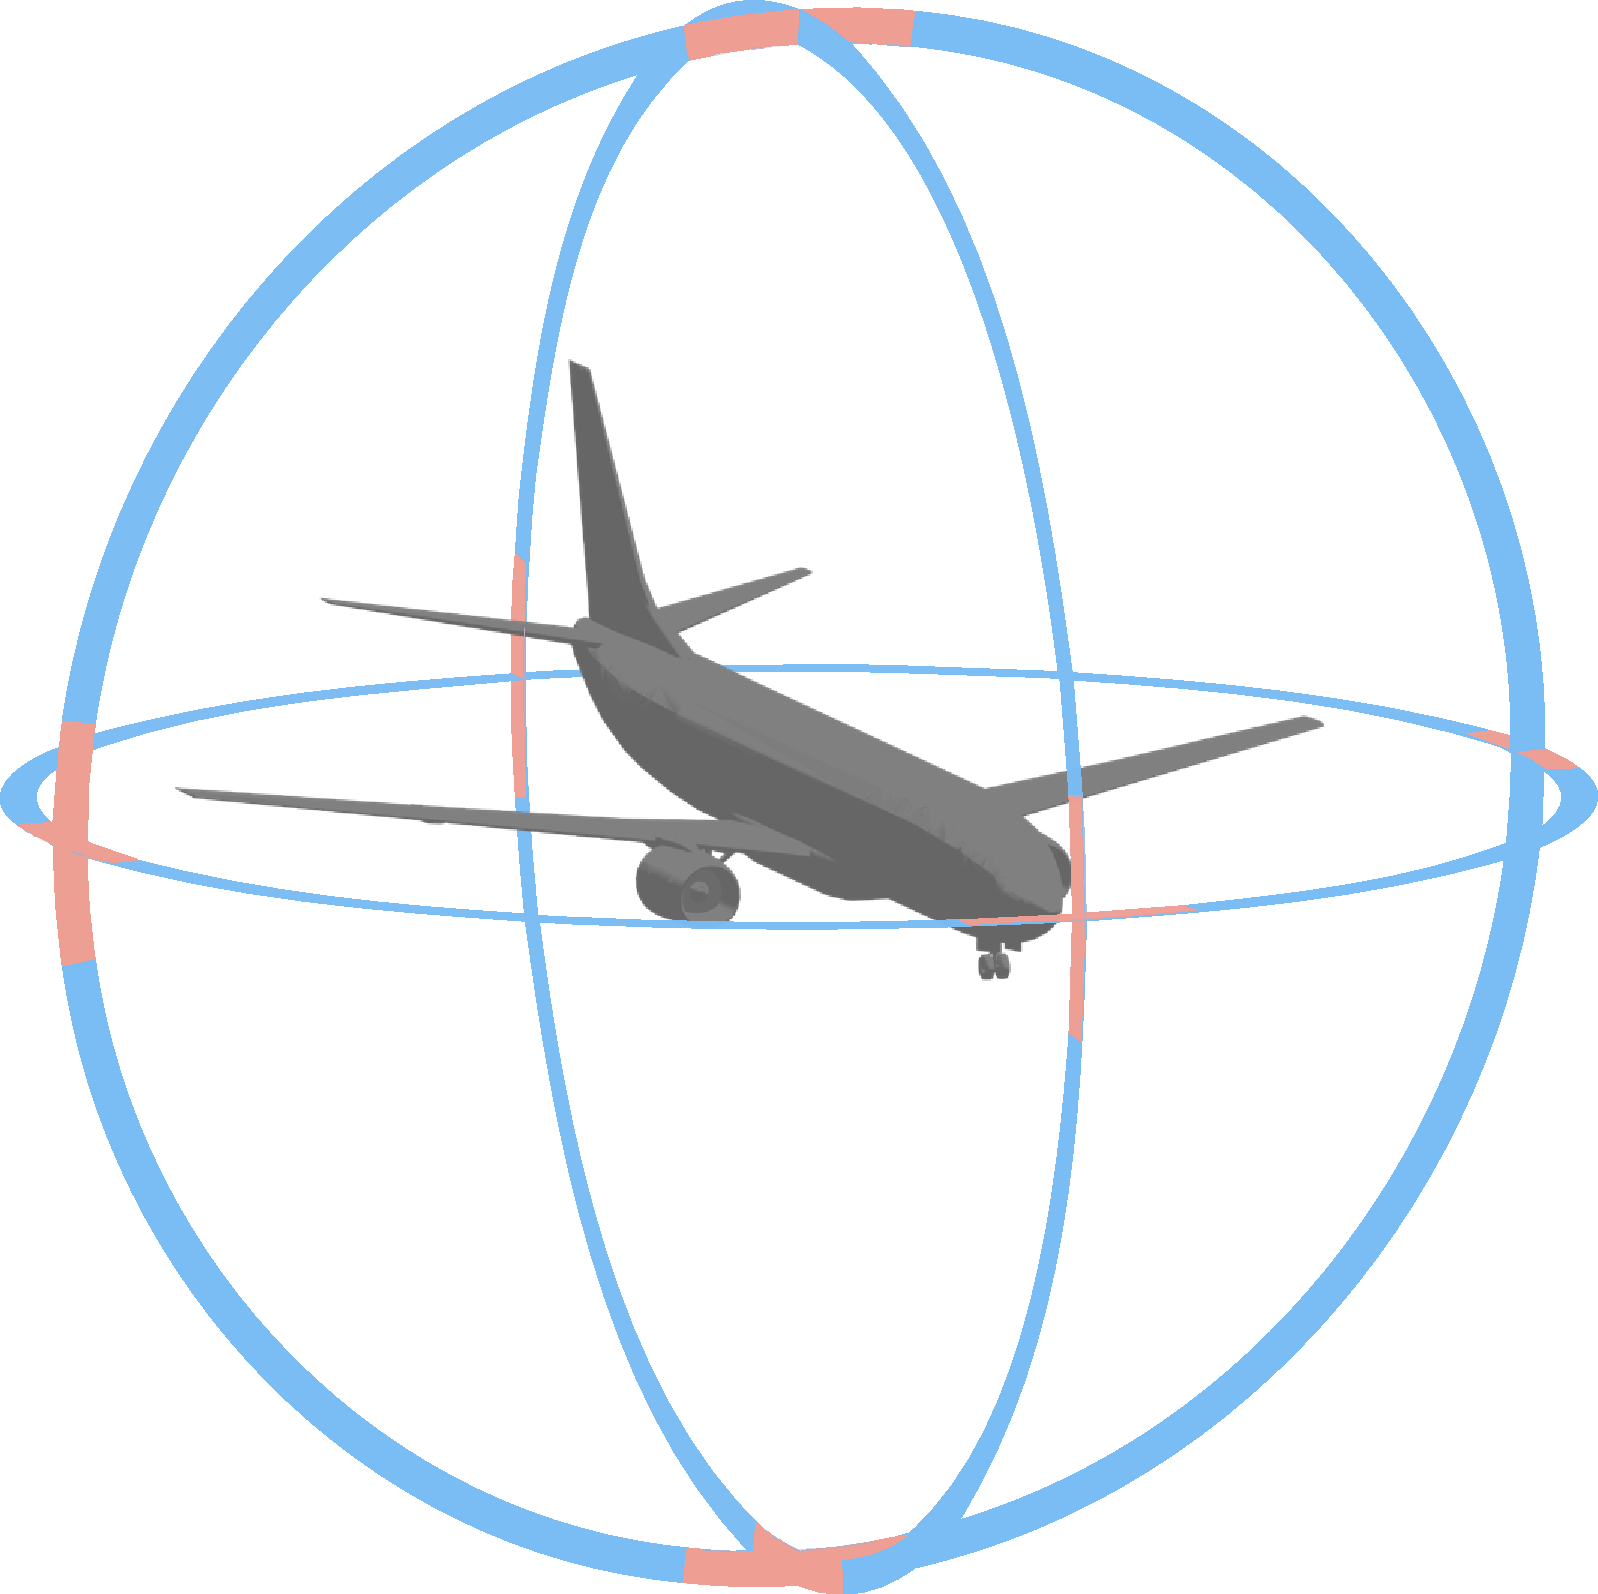
\includegraphics[width=\linewidth]{figures/airplane/so3/airplane.pdf}}
\caption{Range-Gap Vis.}\label{fig:so3_range}
\end{subfigure}
\hfill
\begin{subfigure}{.5\linewidth}
\centering
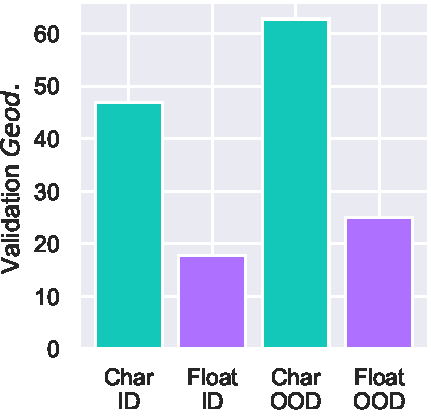
\includegraphics[width=\linewidth]{figures/airplane/so3/bar.pdf}
\caption{ID--OOD}\label{fig:so3_bar}
\end{subfigure}
\caption{\textbf{SO(3) Range Gap.} (\cref{sssec:so3})
(a) Visualization of the SO(3) range-gap sampling space.
For training, Euler rotation components are sampled from the blue regions.
In OOD, samples are exclusively sampled from the red ranges.
(b) The float-based model outperforms the char-based variant on validation data sampled from both the ID and OOD conditions. 
}
\label{fig:so3}
\vspace{-0.5cm}
\end{wrapfigure}